\documentclass{article}
\usepackage[utf8]{inputenc}
\usepackage[justification=centering]{caption}
\usepackage{minted}
\usepackage{graphicx}
\usepackage{amsfonts}
\usepackage{pgfplots}
\usepackage{mathtools}

\renewcommand{\listfigurename}{Table des figures}
\RecustomVerbatimEnvironment{Verbatim}{BVerbatim}{}


\title{MTS211::DM1 \\ Simulation de processus stochastiques}
\author{Maxime Mouchet}
\date{Septembre 2015}

\begin{document}

\maketitle

\section{Généralités}

\begin{itemize}
\item Un vecteur désigne une matrice avec une ligne et $N$ colonnes.
\item Les formules sont données dans le cas continu.
\end{itemize}


\section{Simulation de trajectoires}

\subsection*{Question 1}
Chaque ligne \texttt{x1(w,:)} de \texttt{x1} contient, après simulation, une trajectoire du processus $X_1$. Soit l'ensemble des échantillons pour une réalisation du processus.

\subsection*{Question 2}
Chaque colonne \texttt{x1(:,t)} de \texttt{x1} contient, après simulation, l'échantillon à un instant $t$ du processus $X_1$, pour chacune de chacune de ses réalisations.

\subsection*{Question 3}
Le vecteur \texttt{a} contient l'amplitude des signaux pour chaque échantillon. \\
La fonction \texttt{randn(M,N)} permet de générer une matrice de dimension $M \times N$ constituées de réels pseudo-aléatoires, distribués selon une loi normale centrée réduite. Ici on obtient un vecteur dont le nombre de colonnes est égal au nombre d'échantillons. \\
On multiplie chaque amplitude par l'écart-type $\sigma_a$ et on ajoute la moyenne $\mu_a$ afin d'obtenir la loi normale $\mathcal{N}(\mu_a,\sigma_a)$ désirée à partir de la version réduite :
\begin{figure}[h]
\centering
\begin{minted}{matlab}
a = (randn(1, nRealisation)) * sigma_a + eta_a;
\end{minted}
\end{figure}

\subsection*{Question 4}
Les vecteurs \texttt{phi\_1} et \texttt{phi\_2} contiennent la phase des signaux $X_1$ et $X_2$ pour chaque échantillon. Leur nombre de colonnes est égal au nombre d'échantillons. \\
Pour $X_1$ on définit une phase constante $\mathit{Arg}(X_1) = \frac{\pi}{4}$ à l'aide la fonction \texttt{ones(M,N)} qui permet de générer une matrice constituée de $1$ et en multipliant chaque valeur par la phase désirée :
\begin{figure}[h]
\centering
\begin{minted}{matlab}
phi_1 = ones(1, nRealisation) * pi / 4;
\end{minted}
\end{figure}

\noindent
Pour $X_2$ on définit une phase aléatoire distribuée uniformément dans $[0;2\pi]$ à l'aide de la fonction \texttt{rand} donc le fonctionnement est similaire à la fonction \texttt{randn} à la distribution près :
\begin{figure}[h]
\centering
\begin{minted}{matlab}
phi_2 = rand(1, nRealisation) * 2 * pi;
\end{minted}
\end{figure}

\subsection*{Question 5}

\begin{figure}[h!]
\hspace*{-0.8cm}
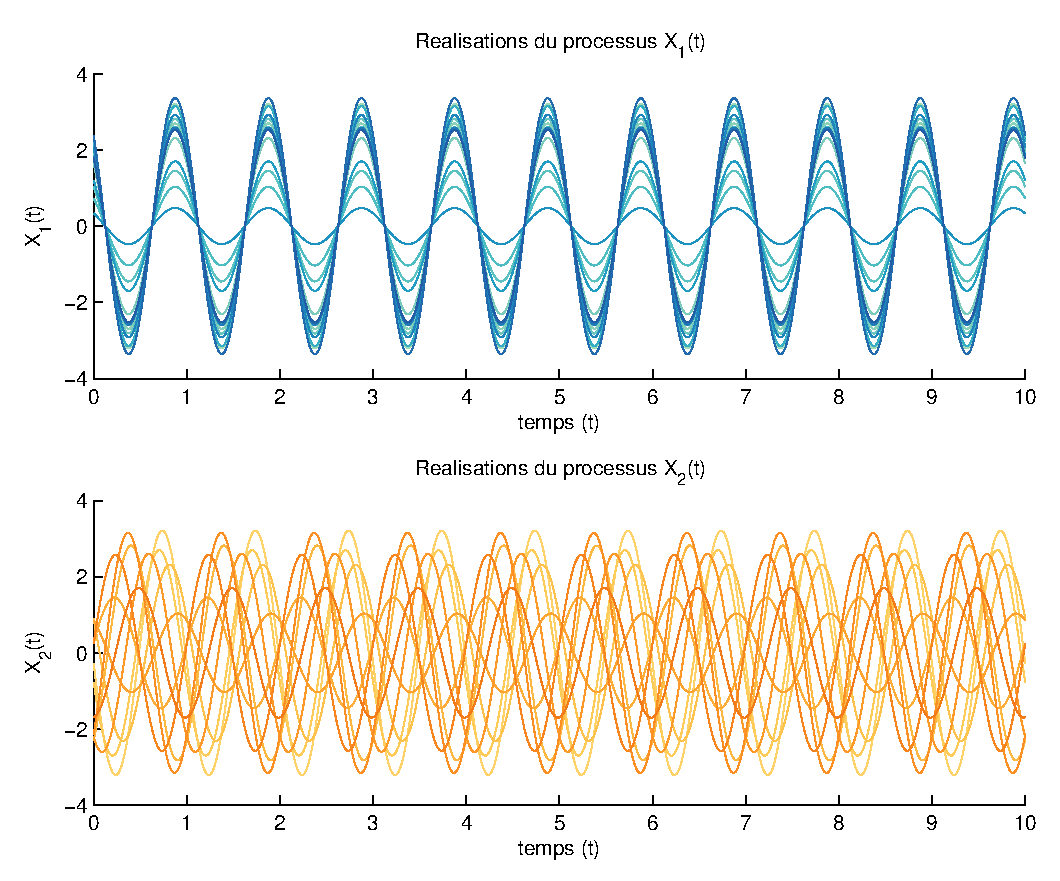
\includegraphics[width=12cm]{q5.eps}
\caption{10 réalisations des processus $X_1$ et $X_2$.}
\end{figure}

La superposition des réalisations du processus $X_1$ met en évidence la variation de l'amplitude des sinus (aléatoire) qui sont tous en phase (phase constante de $\frac{\pi}{4}$). Les zones les plus denses pour $\mathit{cos} = 1$ sont situées aux alentours de 2, ce qui correspond à la valeur moyenne de la loi normale utilisée pour générer l'amplitude.

La superposition des réalisations du processus $X_2$ met en évidence la variation de l'amplitude des sinus et du déphasage, tout les deux aléatoires.

\section{Estimation des moyennes d'ordre 1}

\subsection*{Question 10}
Les vecteurs \texttt{moy\_stat1} et \texttt{moy\_stat2} contiennent respectivement les moyennes statistiques (ou d'ensemble) des processus $X_1$ et $X_2$ pour chaque instant. \\
Leur nombre de colonnes est égal au nombre d'échantillons puisque la moyenne d'ensemble est la moyenne des réalisations du processus à un instant donné.


\subsection*{Question 11}
On affiche la moyenne statistique en fonction du temps des processus $X_1(t)$ et $X_2(t)$ pour 50 (figure \ref{fig:moystat50}) et 500 réalisations (figure \ref{fig:moystat500}). On constate que plus le nombre de réalisations est important, plus la moyenne statistique simulée se rapproche de la moyenne statistique théorique (voir question 12).

Avec un faible de nombre de réalisations, comme pour la figure \ref{fig:moystat50}, on remarque le comportement aléatoire gaussien de l'amplitude en lançant plusieurs fois la simulation successivement. On obtiendra parfois une amplitude maximale pour la moyenne statistique de $X_1$ qui est inférieure à 2, et parfois une amplitude maximale supérieure à 2. Naturellement ce comportement s'estompe avec le nombre de réalisations et pour un grand nombre, comme pour la figure \ref{fig:moystat500}, on tend vers la moyenne théorique de 2.

\begin{figure}[p]
\hspace*{-1.6cm}
\includegraphics[width=15cm]{q11_1.eps}
\caption{Moyenne statistique en fonction du temps des processus $X_1$ et $X_2$ pour 50 réalisations.}
\label{fig:moystat50}
\end{figure}

\begin{figure}[p]
\hspace*{-1.6cm}
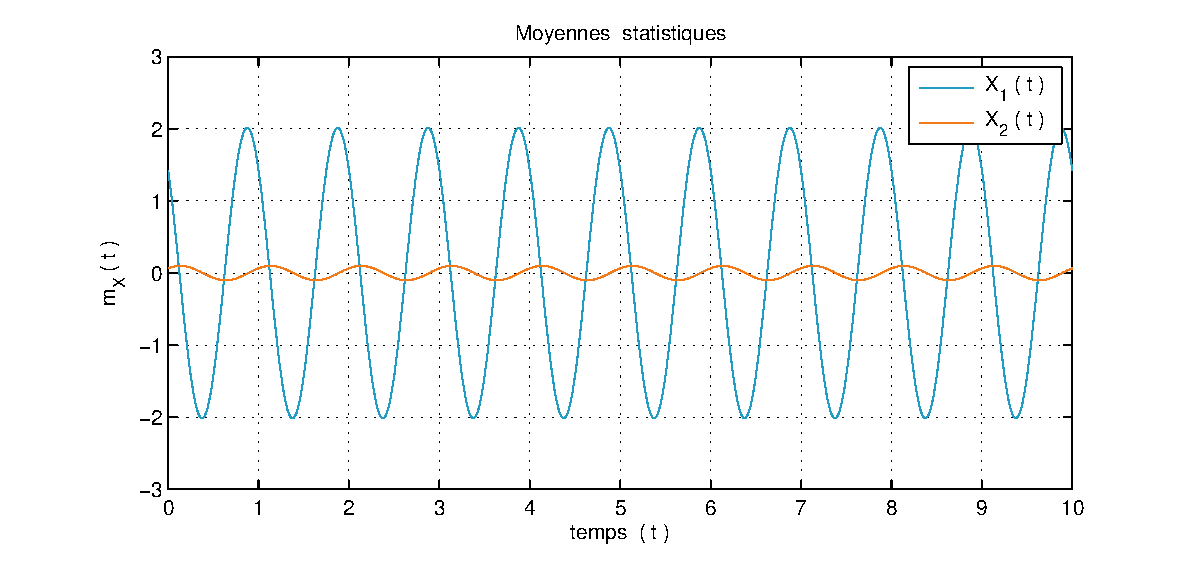
\includegraphics[width=15cm]{q11_2.eps}
\caption{Moyenne statistique en fonction du temps des processus $X_1$ et $X_2$ pour 500 réalisations.}
\label{fig:moystat500}
\end{figure}

\newpage
\subsection*{Question 12}
On calcule la moyenne statistique de $X_1$ :

\begin{equation}
\begin{aligned}
m_{X_1}(t)
& = \mathbb{E}\{(X_1(t))\} \\ 
& = \mathbb{E}\{a(\omega).\cos(2\pi\nu t+\phi)\} \\
& = \mathbb{E}\{a(\omega)\}.\cos(2\pi\nu t+\phi) \\
& = 2\cos(2\pi\nu t+\phi)
\end{aligned}
\end{equation}

\noindent
La moyenne statistique de $X_1$ est dépendante du temps. On retrouve ce comportement sur la moyenne statistique simulé (figure \ref{fig:moystat50} et \ref{fig:moystat500}) avec une courbe sinusoïdale.

\noindent
On calcule la moyenne statistique de $X_2$, $a$ et $\phi$ sont indépendantes :

\begin{equation}
\begin{aligned}
m_{X_2}(t)
& = \mathbb{E}\{(X_2(t))\} \\
& = \mathbb{E}\{a(\omega)\cos(2\pi\nu t+\phi(\omega))\} \\
& = 2.\mathbb{E}\{\cos(2\pi\nu t+\phi(\omega))\} \\
& = 2.\mathbb{E}\{\cos(2\pi\nu t)\cos(\phi(\omega)) - \sin(2\pi\nu t)\sin(\phi(\omega))\} \\
& = 2.[\mathbb{E}\{\cos(\phi(\omega))\}\cos(2\pi\nu t) - \mathbb{E}\{\sin(\phi(\omega))\sin(2\pi\nu t)\}] \\
& = 2.[0\cos(2\pi\nu t) - 0\sin(2\pi\nu t)] \\
& = 0
\end{aligned}
\end{equation}

\noindent
Le processus $X_2$ est centré et sa moyenne ne dépend pas du temps. On retrouve ce comportement sur la moyenne statistique simulé (figure \ref{fig:moystat50} et \ref{fig:moystat500}) où la courbe tend vers une droite $y = 0$ pour un grand nombre de réalisations.

\subsection*{Question 13}
Un processus est stationnaire à l'ordre 1 si sa moyenne statistique ne dépend pas du temps : 
\begin{equation*}
m_X(t) = m_X = \mathit{cte.}
\end{equation*}

\noindent
C'est le cas du processus $X_2$ ($m_X(t) = 0$) mais pas du processus $X_1(t)$ ($m_X(t) = 2\cos(2\pi\nu t+\phi)$). \\
On vérifie ce comportement sur les simulations. En effet, pour un grand nombre de réalisations, la courbe de la moyenne statistique de $X_2$ (stationnaire) tend vers une droite (constante), alors que la courbe de la moyenne de $X_1$ (non stationnaire) a toujours une allure sinusoïdale (dépendante du temps).

\subsection*{Question 15}
Les vecteurs \texttt{moy\_temp1} et \texttt{moy\_temp2} contiennent respectivement les moyennes temporelles des processus $X_1$ et $X_2$ pour chaque réalisation. Leur nombre de colonnes est égal au nombre de réalisations puisqu'il y a une moyenne temporelle par réalisation.

\subsection*{Question 16}
\begin{figure}[h]
\centering
\includegraphics[width=12cm]{q16.eps}
\caption{Moyenne temporelle en fonction de la réalisation\\des processus $X_1$ et $X_2$ pour 500 réalisations.}
\label{fig:moytemp}
\end{figure}


\subsection*{Question 17}
\begin{equation}
\begin{aligned}
\overline{X_1(\omega_0)} & = \lim_{T\rightarrow\infty} \frac{1}{2T}\int_{-T}^{+T}a_0\cos(2\pi\nu t + \phi) dt \\
& = \lim_{T\rightarrow\infty} \frac{a_0}{2T}[\sin(2\pi\nu t + \phi)]_{-T}^{T} \\
& = \lim_{T\rightarrow\infty} \frac{a_0}{2T}[\sin(2\pi\nu T + \phi) - \sin(2\pi\nu (-T) + \phi)] \\
& = 0
\end{aligned}
\end{equation}

\begin{equation}
\begin{aligned}
\overline{X_2(\omega_0)} & = \lim_{T\rightarrow\infty} \frac{1}{2T}\int_{-T}^{+T}a_0\cos(2\pi\nu t + \phi_0) dt \\
& = \lim_{T\rightarrow\infty} \frac{a_0}{2T}[\sin(2\pi\nu t + \phi_0)]_{-T}^{T} \\
& = \lim_{T\rightarrow\infty} \frac{a_0}{2T}[\sin(2\pi\nu T + \phi_0) - \sin(2\pi\nu (-T) + \phi_0)] \\
& = 0
\end{aligned}
\end{equation}

\noindent
Les valeurs de 0 calculées pour la moyenne temporelle sont très proches (à $10^{-3}$ près) des valeurs mesurées sur la figure \ref{fig:moytemp}.

\subsection*{Question 18}
Un processus est ergodique à l'ordre 1 si sa moyenne temporelle est indépendante de la réalisation :
\begin{equation*}
\overline{X(\omega_0)} = \overline{X} = \mathit{cte.}
\end{equation*}

\noindent
C'est le cas des processus $X_1$ et $X_2$ (cf. moyennes temporelles calculées à la question 17). \\
On vérifie cela sur la figure \ref{fig:moytemp} par la très faible dispersion ($\pm 4\times10^{-3}$) des valeurs autour de la moyenne temporelle théorique en fonction de la réalisation.

\subsection*{Question 20}
Un processus est de moyenne ergodique si il est stationnaire à l'ordre 1 et que sa moyenne d'ensemble est égale à sa moyenne temporelle :
\begin{equation*}
\mathbb{E}\{X(t,\omega)\} = \lim_{T\rightarrow\infty}\frac{1}{2T}\int_{-T}^{+T}X(t,\omega)dt = \mathit{cte.}
\end{equation*}

\noindent
Ce n'est pas le cas du processus $X_1$ :
\begin{equation*}
\mathbb{E}\{(X_1(t))\} = 2\cos(2\pi\nu t+\phi) \neq \overline{X_1(\omega_0)} = 0
\end{equation*}

\noindent
Mais c'est le cas pour le processus $X_2$ :
\begin{equation*}
\mathbb{E}\{(X_2(t))\} = \overline{X_2(\omega_0)} = 0
\end{equation*}

\noindent
On vérifie cela sur les figures \ref{fig:moystat500} et \ref{fig:moytemp} où pour un grand nombre de réalisations la moyenne statistique de $X_2$ se rapproche de sa moyenne temporelle de 0.

\section{Autocorrélation d'un processus stochastique}


\subsection*{Question 30}
Les matrices \texttt{gamma1} et \texttt{gamma2} contiennent l'autocorrélation statistique estimée pour les processus $X_1$ et $X_2$. Chaque ligne représente un échantillon temporel $t$ et chaque colonne correspond à un pas $\tau$. La cellule $(t,\tau)$ contient donc la valeur de l'autocorrélation $\Gamma_X(t,t+\tau)$. \\
Leur nombre de lignes est égal au nombre d'échantillons moins l'écart considéré (sinon on dépasserait le nombre d'échantillons). Leur nombre de colonnes est égal au nombre de pas considéré, puisque chaque colonne représente un pas $\tau$.

\newpage
\subsection*{Question 31}
 ~ 
\begin{figure}[!h]
\hspace*{-2cm}
%\centerline
\includegraphics[width=18cm]{q31_bis.eps}
\caption{Autocorrélation statistique estimée pour les processus $X_1$ et $X_2$.}
\label{fig:autocorrstat}
\end{figure}

\subsection*{Question 32}

\begin{equation}
\begin{aligned}
\Gamma_{X_1}(t,t+\tau)
& = \mathbb{E}\{X_1(t)X_1^*(t+\tau)\} \\
& = \mathbb{E}\{a(\omega).\cos(2\pi\nu t + \phi).a(\omega).\cos(2\pi\nu(t+\tau) + \phi)\} \\
& = \mathbb{E}\{a(\omega)^2\}.\cos(2\pi\nu t + \phi).\cos(2\pi\nu(t+\tau) + \phi) \\
& = (\sigma^2 + \mu^2).g(t,\tau) = 5.g(t,\tau)
\end{aligned}
\end{equation}

\noindent
On remarque que la fonction d'autocorrélation de $X_1$ est dépendante du temps $t$ et du décalage $\tau$. On retrouve ce comportement sur la figure \ref{fig:autocorrstat} où le déplacement sur l'un des deux axes fait varier la valeur. De plus on retrouve les valeurs minimum (bleu) et maximum (rouge) de $-5$ et $5$ lorsque le produit de cosinus vaut $-1$ ou $1$.

\noindent
Pour $\Gamma_{X_2}$ on sait que  $a$ et $\phi$ sont indépendants. On a donc :
\begin{equation}
\begin{aligned}
\Gamma_{X_2}(t,t+\tau)
& = \mathbb{E}\{X_2(t)X_2^*(t+\tau)\} \\
& = \int_{\mathcal{D}_a}\int_{\mathcal{D}_\phi}a(\omega).\cos(2\pi\nu t + \phi(\omega)).a(\omega).\cos(2\pi\nu(t+\tau) + \phi(\omega)).f_{a,\phi}(a,\phi)\mathit{da}\mathit{d\phi} \\
& = \int_{\mathcal{D}_a}a(\omega)^2.f_a(a)da.\int_{\mathcal{D}_\phi}\cos(2\pi\nu t + \phi(\omega)).\cos(2\pi\nu(t+\tau) + \phi(\omega)).f_{\phi}(\phi)d\phi \\
& = \mathbb{E}\{a(\omega)^2\}.\int_0^{2\pi}\frac{1}{2\pi}\frac{\cos(4\pi\nu t + 2\pi\nu\tau + 2\phi) + \cos(2\pi\nu\tau)}{2}d\phi \\
& = \mathbb{E}\{a(\omega)^2\}.[\frac{1}{4\pi}\int_0^{2\pi}\cos(4\pi\nu t + 2\phi)d\phi + \frac{\cos(2\pi\nu\tau)}{4\pi}\int_0^{2\pi}d\phi] \\
& = \frac{(\sigma^2 +\mu^2)}{2}.cos(2\pi\nu\tau) = \frac{5}{2}.cos(2\pi\nu\tau)
\end{aligned}
\end{equation}

\noindent
On remarque que la fonction d'autocorrélation de $X_2$ ne dépend que du décalage $\tau$. On retrouve ce comportement sur la figure \ref{fig:autocorrstat} où seul le déplacement sur l'axe des abscisses (décalage $\tau$) fait varier la valeur de l'autocorrélation. De la même façon que pour $X_1$, on retrouve les valeurs minimum et maximum de $-2.5$ et $2.5$ lorsque le cosinus vaut $-1$ ou $1$.

\subsection*{Question 33}
Un processus est stationnaire à l'ordre 2 (SSL) si sa moyenne statistique ne dépend pas du temps et si sa fonction d'autocorrélation ne dépend que de la différence entre les deux instants considérés :
\begin{itemize}
\item $m_X(t) = m_X = \mathit{cte}$
\item $\Gamma_X(t_1,t_2) = \mathbb{E}\{X(t_1)X(t_2)^*\} = \Gamma_X(t_1 - t_2)$
\end{itemize}

\noindent
$X_1$ n'est pas stationnaire à l'ordre 2 puisque sa moyenne statistique (cf. question 12) et sa fonction d'autocorrélation (cf. question 32) sont dépendantes du temps.
~ \\
\noindent
Au contraire, $X_2$ est stationnaire à l'ordre 2. Sa moyenne statistique et sa fonction d'autocorrélation ne dépendent pas du temps. On observe cela sur le tracé de l'autocorrélation statistique (figure \ref{fig:autocorrstatx2}) qui est une surface qui est ne varie qu'en fonction du décalage $\tau$ et pas de l'instant $t$.

\begin{figure}[h]
\includegraphics[width=12cm]{q33.eps}
\caption{Autocorrélation statistique estimée pour le processus $X_2$. Mise en évidence de la stationnarité d'ordre 2.}
\label{fig:autocorrstatx2}
\end{figure}

\subsection*{Question 35}
Les matrices \texttt{auto1} et \texttt{auto2} contiennent l'autocorrélation temporelle estimée pour les processus $X_1$ et $X_2$. Chaque ligne représente une trajectoire $\omega$ et chaque colonne correspond à un pas $\tau$. La cellule $(\omega,\tau)$ contient donc la valeur de l'autocorrélation $\overline{X(\omega,t)X(\omega,t+\tau)^*}$. \\
Leur nombre de lignes est égal au nombre de réalisations, puisqu'une ligne représente une trajectoire. Leur nombre de colonnes est égal au nombre d'échantillons plus 1.

\subsection*{Question 36}
\begin{figure}[!h]
\hspace*{-1.25cm}
\includegraphics[width=15cm]{q35.eps}
\caption{Autocorrélation temporelle estimée pour les processus $X_1$ et $X_2$.}
\label{fig:autocorrtempx1x2}
\end{figure}

\subsection*{Question 37}

\begin{equation}
\begin{aligned}
\overline{X_1(\omega,t)X_1(\omega,t+\tau)^*}
& = \lim_{T\rightarrow\infty} \frac{1}{2T}\int_{-T}^{+T}X_1(\omega,t)X_1(\omega,t+\tau)^*dt \\
& = \lim_{T\rightarrow\infty} \frac{1}{2T}\int_{-T}^{+T} a_0\cos(2\pi\nu t +\phi)a_0\cos(2\pi\nu(t-\tau) +\phi)) dt \\
& = \lim_{T\rightarrow\infty} \frac{a_0^2}{2T}\int_{-T}^{+T} \frac{1}{2}[\cos(4\pi\nu t + 2\pi\nu\tau + 2\phi) + \cos(2\pi\nu\tau)] dt \\
& = \lim_{T\rightarrow\infty} \frac{a_0^2}{4T} [\int_{-T}^{+T} \cos(4\pi\nu t + 2\pi\nu\tau + 2\phi) dt + \cos(2\pi\nu\tau) \int_{-T}^{+T} dt] \\
& = \lim_{T\rightarrow\infty} \frac{a_0^2}{4T.4\pi\nu}[\sin(4\pi\nu t + 2\pi\nu\tau + 2\phi)]_{-T}^T + \lim_{T\rightarrow\infty} \frac{a_0^2\cos(2\pi\nu\tau)2T}{4T} \\
& = \frac{a_0^2\cos(2\pi\nu\tau)}{2}
\end{aligned}
\end{equation}

Pour $X_2$ on remplace $\phi$ par $\phi_0$ puisque la phase de ce signal est aléatoire et on obtient le même résultat que pour $X_1$ :

\begin{equation}
\begin{aligned}
\overline{X_2(\omega,t)X_2(\omega,t+\tau)^*}
& = \frac{a_0^2\cos(2\pi\nu\tau)}{2}
\end{aligned}
\end{equation}

On retrouve $a_0$ dans la valeur de l'autocorrélation temporelle calculée pour $X_1$ et $X_2$, elle dépend donc de la trajectoire pour ces deux processus.

\subsection*{Question 38}
Un processus est ergodique à l'ordre 2 si sa fonction d'autocorrélation temporelle est indépendante de la trajectoire choisie :
\begin{equation*}
\overline{X(\omega,t)X(\omega,t+\tau)^*} = \overline{X(t)X(t+\tau)^*}
\end{equation*}

\noindent
Ce n'est pas le de cas $X_1$ et $X_2$ (cf. question 37). On retrouve la dépendance à la trajectoire sur la figure \ref{fig:autocorrtempx1x2} puisqu'un déplacement sur l'axe des ordonnées fait varier la valeur de l'autocorrélation.

\subsection*{Question 40}
Un processus est de corrélation ergodique si sa fonction d'autocorrélation statistique est égale à sa fonction d'autocorrélation temporelle :
\begin{equation*}
\Gamma_X(\tau) = \lim_{T\rightarrow\infty}\frac{1}{2T}\int_{-T}^{+T}X(t,\omega_0)X^*(t-\tau,\omega_0)dt
\end{equation*}

\noindent
Ce n'est pas le cas de $X_1$ et $X_2$ puisque leurs fonctions d'autocorrélation statistiques et temporelles ne sont pas égales (cf. question 32 et 37). On vérifie cela sur la visualisation des autocorrélations statistiques et temporelles estimées, puisque l'on n'observe pas le même motif.

\section{Processus ergodique}

\subsection*{Question 50}
On considère maintenant $\boldsymbol{a}$ comme une valeur déterministe égale à $2$.
\noindent
$X_1$ devient un signal déterministe :
\begin{equation*}
X_1(t) = \boldsymbol{a}.\cos(2\pi\nu t + \phi)
\end{equation*}

\noindent
$X_2$ devient un signal dont la phase est la seule composante aléatoire :
\begin{equation*}
X_2(t,\omega) = \boldsymbol{a}.\cos(2\pi\nu t + \phi(\omega))
\end{equation*}

\subsubsection*{Calcul de la moyenne statistique}

\begin{equation}
\begin{aligned}
m_{X_1}(t) = 2.\cos(2\pi\nu t + \phi)
\end{aligned}
\end{equation}

\begin{equation}
\begin{aligned}
m_{X_2}(t)
& = \mathbb{E}\{\boldsymbol{a}.\cos(2\pi\nu t+\phi(\omega))\} \\
& = 2.[0\cos(2\pi\nu t) - 0\sin(2\pi\nu t)] \\
& = 0
\end{aligned}
\end{equation}

\noindent
On retrouve les mêmes conclusions que lorsque $a$ était une variable aléatoire : $X_1$ n'est pas stationnaire à l'ordre 1 mais $X_2$ l'est (moyenne statistique constante).

\subsubsection*{Calcul de la moyenne temporelle}

\begin{equation}
\begin{aligned}
\overline{X_1(\omega_0)} & = \lim_{T\rightarrow\infty} \frac{1}{2T}\int_{-T}^{+T}\boldsymbol{a}\cos(2\pi\nu t + \phi) dt \\
& = \lim_{T\rightarrow\infty} \frac{\boldsymbol{a}}{2T}[\sin(2\pi\nu t + \phi)]_{-T}^{T} \\
& = \lim_{T\rightarrow\infty} \frac{\boldsymbol{a}}{2T}[\sin(2\pi\nu T + \phi) - \sin(2\pi\nu (-T) + \phi)] \\
& = 0
\end{aligned}
\end{equation}

\begin{equation}
\begin{aligned}
\overline{X_2(\omega_0)} & = \lim_{T\rightarrow\infty} \frac{1}{2T}\int_{-T}^{+T}\boldsymbol{a}\cos(2\pi\nu t + \phi_0) dt \\
& = \lim_{T\rightarrow\infty} \frac{\boldsymbol{a}}{2T}[\sin(2\pi\nu t + \phi_0)]_{-T}^{T} \\
& = \lim_{T\rightarrow\infty} \frac{\boldsymbol{a}}{2T}[\sin(2\pi\nu T + \phi_0) - \sin(2\pi\nu (-T) + \phi_0)] \\
& = 0
\end{aligned}
\end{equation}

\noindent
Logiquement les résultats n'ont pas changé puisque l'amplitude n'affecte pas la moyenne d'un signal sinusoïdal (si il n'y a pas de composante continue). On retrouve les mêmes conclusions qu'à la question 20 : $X_2$ est de moyenne ergodique, mais pas $X_1$.

\subsubsection*{Calcul de l'autocorrélation statistique}

\begin{equation}
\begin{aligned}
\Gamma_{X_1}(t,t+\tau)
& = \mathbb{E}\{X_1(t)X_1^*(t+\tau)\} \\
& = \mathbb{E}\{\boldsymbol{a}.\cos(2\pi\nu t + \phi).\boldsymbol{a}.\cos(2\pi\nu(t+\tau) + \phi)\} \\
& = \boldsymbol{a^2}.\cos(2\pi\nu t + \phi).\cos(2\pi\nu(t+\tau) + \phi) \\
& = \boldsymbol{a^2}.g(t,\tau) = 4.g(t,\tau)
\end{aligned}
\end{equation}

\begin{equation}
\begin{aligned}
\Gamma_{X_2}(t,t+\tau)
& = \mathbb{E}\{X_2(t)X_2^*(t+\tau)\} \\
& = \int_{\mathcal{D}_\phi}\boldsymbol{a}.\cos(2\pi\nu t + \phi(\omega)).\boldsymbol{a}.\cos(2\pi\nu(t+\tau) + \phi(\omega)).f_{\phi}(\phi)\mathit{d\phi} \\
& = \boldsymbol{a^2}.\int_{\mathcal{D}_\phi}\cos(2\pi\nu t + \phi(\omega)).\cos(2\pi\nu(t+\tau) + \phi(\omega)).f_{\phi}(\phi)d\phi \\
& = \boldsymbol{a^2}.\int_0^{2\pi}\frac{1}{2\pi}\frac{\cos(4\pi\nu t + 2\pi\nu\tau + 2\phi) + \cos(2\pi\nu\tau)}{2}d\phi \\
& = \boldsymbol{a^2}.[\frac{1}{4\pi}\int_0^{2\pi}\cos(4\pi\nu t + 2\phi)d\phi + \frac{\cos(2\pi\nu\tau)}{4\pi}\int_0^{2\pi}d\phi] \\
& = \frac{4}{2}.cos(2\pi\nu\tau) = 2.cos(2\pi\nu\tau)
\end{aligned}
\end{equation}

\noindent
On retrouve les mêmes conclusions qu'à la question 33. $X_2$ est stationnaire à l'ordre 2, mais pas $X_1$.

\subsubsection*{Calcul de l'autocorrélation temporelle}

\begin{equation}
\begin{aligned}
\overline{X_1(\omega,t)X_1(\omega,t+\tau)^*}
& = \lim_{T\rightarrow\infty} \frac{1}{2T}\int_{-T}^{+T}X_1(\omega,t)X_1(\omega,t+\tau)^*dt \\
& = \lim_{T\rightarrow\infty} \frac{1}{2T}\int_{-T}^{+T} \boldsymbol{a}\cos(2\pi\nu t +\phi)\boldsymbol{a}\cos(2\pi\nu(t-\tau) +\phi)) dt \\
& = \lim_{T\rightarrow\infty} \frac{\boldsymbol{a^2}}{2T}\int_{-T}^{+T} \frac{1}{2}[\cos(4\pi\nu t + 2\pi\nu\tau + 2\phi) + \cos(2\pi\nu\tau)] dt \\
& = \lim_{T\rightarrow\infty} \frac{\boldsymbol{a^2}}{4T} [\int_{-T}^{+T} \cos(4\pi\nu t + 2\pi\nu\tau + 2\phi) dt + \cos(2\pi\nu\tau) \int_{-T}^{+T} dt] \\
& = \lim_{T\rightarrow\infty} \frac{\boldsymbol{a^2}}{4T.4\pi\nu}[\sin(4\pi\nu t + 2\pi\nu\tau + 2\phi)]_{-T}^T + \lim_{T\rightarrow\infty} \frac{\boldsymbol{a^2}\cos(2\pi\nu\tau)2T}{4T} \\
& = \frac{4}{2}.\cos(2\pi\nu\tau) = 2.\cos(2\pi\nu\tau)
\end{aligned}
\end{equation}

Pour $X_2$ on remplace $\phi$ par $\phi_0$ puisque la phase de ce signal est aléatoire et on obtient le même résultat que pour $X_1$ :

\begin{equation}
\begin{aligned}
\overline{X_2(\omega,t)X_2(\omega,t+\tau)^*}
& = 2\cos(2\pi\nu\tau)
\end{aligned}
\end{equation}

\noindent
Contrairement à la conclusion de la question 38, les processus sont ergodiques à l'ordre 2 puisque leur autocorrélation temporelle ne dépend pas de la trajectoire. \\
On remarque également que l'autocorrélation temporelle de $X_2$ est égale à son autocorrélation statistique. Ce processus est donc de corrélation ergodique.

\subsection*{Question 51}

On relance les simulations en fixant $a$ à $2$ :
\begin{minted}{matlab}
a = ones(1, nRealisation) * 2;
\end{minted}

\begin{figure}[h]
\hspace*{-1cm}
%\centerline
\includegraphics[width=14cm]{q51_2.eps}
\caption{Autocorrélation statistique estimée pour les processus $X_1$ et $X_2$ avec $a = 2$.}
\end{figure}

\begin{figure}[h]
\hspace*{-1cm}
%\centerline
\includegraphics[width=14cm]{q51_3.eps}
\caption{Autocorrélation temporelle estimée pour les processus $X_1$ et $X_2$ avec $a = 2$.}
\end{figure}

\newpage
\noindent
On remarque plusieurs changements par rapport aux simulations avec $a(w)$ :
\begin{itemize}
\item Les autocorrélations temporelles de $X_1$ et $X_2$ ne dépendent plus de la trajectoire (motif en bande, confirmé par le calcul).
\item Le motif de l'autocorrélation statistique de $X_2$ est identique à celui de sont autocorrélation temporelle (bandes identiques, confirmé par le calcul). $X_2$ est ergodique.
\end{itemize}

\newpage
\listoffigures
\end{document}
